% !TEX root = ../main.tex

\begin{abstract}
Software systems that learn from data with AI and machine learning (ML) are becoming ubiquitous and are increasingly used to automate impactful decisions. The risks arising from this widespread use of AI/ML are garnering attention from policy makers, scientists, and the media, and lead to the question what data management research can contribute to reduce such risks. 
%
These dangers of AI/ML applications are relatively new and recent, however our societies have had to deal with the dangers of complex and distributed technical processes for a long time already. Based on this insight, we detail how the U.S. Food and Drug Administration (FDA) combats the outbreaks of foodborne illnesses, and use their processes as an inspiration for a data-centric vision towards responsible~AI.

\begin{figure}[h!]
    \centering
    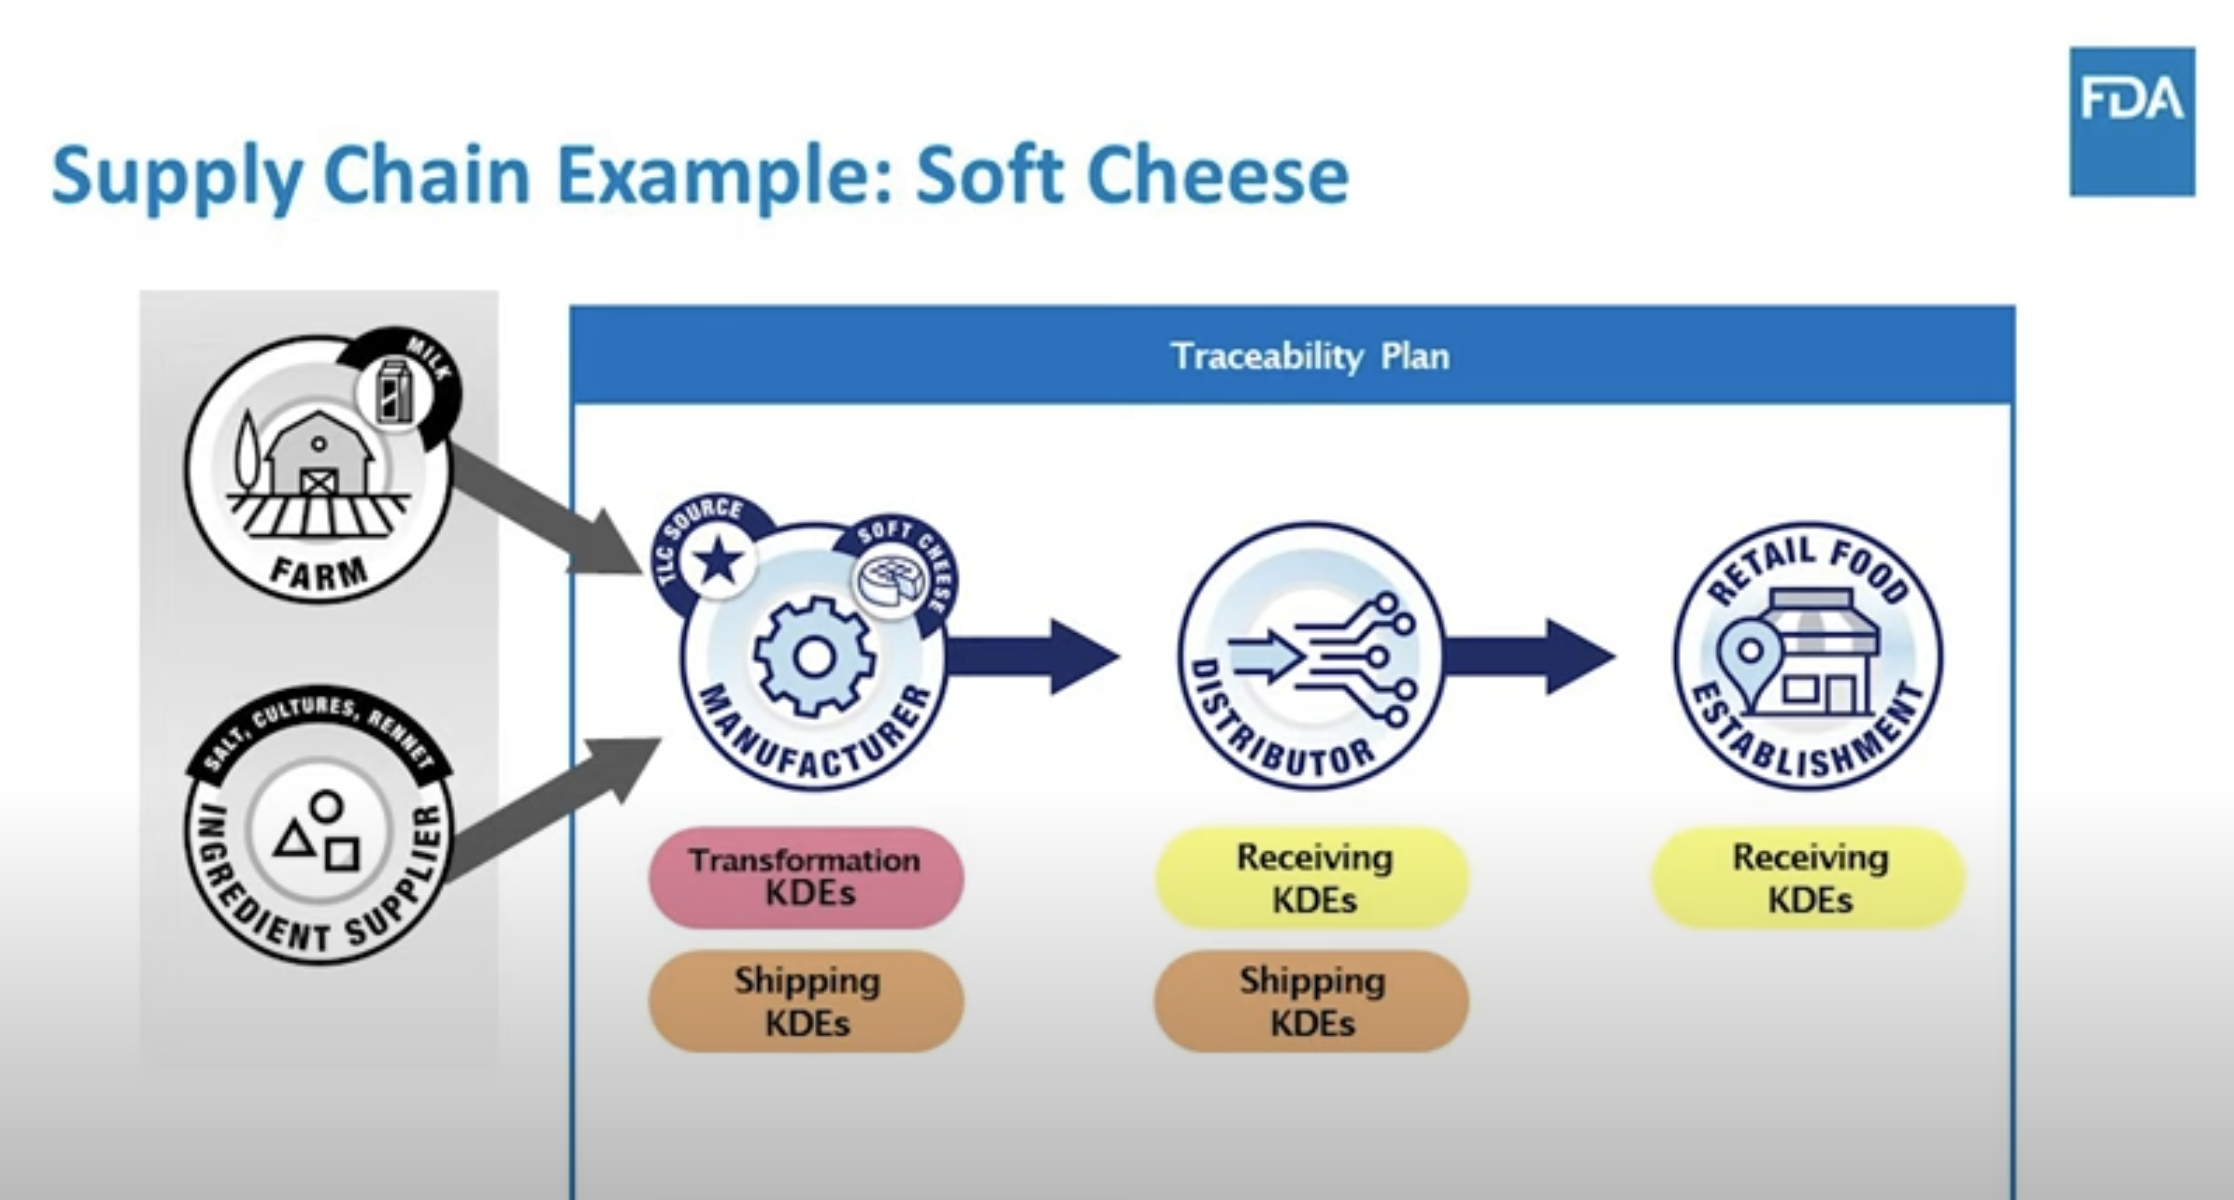
\includegraphics[width=0.6\textwidth]{submissions/submission3/figures/softcheese.png}
    \caption{Food processing is a complex process conducted by different parties in a geo-distributed setting.\protect\footnotemark{} During this process, foods from different sources are joined, transformed from one form to another, and distributed all over the world. At each of these steps, the output could perish and become poisonous, making the final outcome unsafe to consume. \textit{What can we learn from the millennial pursuit of food safety? What type of technical and regulatory frameworks exist such that we trust what we put on the table for our family everyday? And how can we obtain the same level of trust for our data products?}}
\end{figure}

\end{abstract}


\footnotetext{\url{https://www.youtube.com/watch?v=0wnSiC5xqqs}}